\documentclass[12pt]{ctexart}

% 包含必要的包
\usepackage[utf8]{inputenc}
\usepackage{amsmath, amssymb}  % 数学符号包
\usepackage{graphicx}  % 插入图片的包
\usepackage{hyperref}  % 生成超链接
\usepackage{fancyhdr}  % 页眉页脚设置
\usepackage{geometry}  % 页面设置
\usepackage{titlesec}  % 用于自定义 section 的格式
\usepackage{float}
\usepackage{listings}
\usepackage{xcolor}

\geometry{a4paper, margin=1in}

\titleformat{\section}[hang]{\normalfont\Large\bfseries}{\thesection}{1em}{}

\lstset{
    language=Python,
    basicstyle=\ttfamily\small,
    keywordstyle=\color{blue},
    stringstyle=\color{red},
    commentstyle=\color{green!50!black},
    numbers=left,
    numberstyle=\tiny\color{gray},
    frame=single,
    breaklines=true,
    backgroundcolor=\color{gray!10},
    showstringspaces=false,
    % captionpos=b % 让代码标题出现在代码下方
}

% Header and footer
\setlength{\headheight}{14.49998pt}
\addtolength{\topmargin}{-2.49998pt}

\pagestyle{fancy}
\fancyhf{}
\fancyhead[L]{《统计信号处理》实验报告}
% \fancyhead[M]{清华大学}
\fancyhead[R]{刘昱杉 2024214103}
\fancyfoot[C]{\thepage}



\begin{document}

\begin{titlepage}
    \begin{center}
        % Insert logo
        
\includegraphics[width=5cm]{tsinghua_logo.png}\\[4cm]  % 插入图标并设置下方间距
        {\Huge 实验二:信号参量估计与回归} \\[4cm]
        {\large 刘昱杉  \ \  2024214103}\\[6cm]
        {\normalsize \today}\\[1cm]
        \vfill
        \text{注:本实验报告为单人独立完成}\\
        \text{关于本实验报告对应的源码及实验环境,详见\texttt{code}目录下\texttt{readme}}

    \end{center}
\end{titlepage}

\section*{未知幅度(单参量)估值(一)}

\subsection*{1. 实验原理}

假设观测信号模型为:
\[
z_i = A + n_i
\]
其中:
\begin{itemize}
    \item \( A \) 为未知的幅度参数。
    \item \( n_i \) 为均值为0、方差为 \( \sigma^2 \) 的白高斯噪声。
\end{itemize}

最大似然估计方法通过最大化观测数据的似然函数来估计未知参数 \( A \)。对于 \( N \) 次独立采样,似然函数为:
\[
L(A) = \prod_{i=1}^{N} \frac{1}{\sqrt{2\pi\sigma^2}} \exp\left(-\frac{(z_i - A)^2}{2\sigma^2}\right)
\]

取对数似然函数并对 \( A \) 求导,得到最大似然估计量为样本均值:
\[
\hat{A} = \frac{1}{N} \sum_{i=1}^{N} z_i
\]
\begin{itemize}
    \item \textbf{无偏性}:
    \[
    E[\hat{A}] = A
    \]
    \item \textbf{方差}:
    \[
    \text{Var}(\hat{A}) = \frac{\sigma^2}{N}
    \]
\end{itemize}

\subsection*{2. 实验过程与结果}

实验分为三部分:

\begin{enumerate}
    \item \textbf{实验1}:采样次数 \( N = 10 \),噪声方差 \( \sigma^2 = 0.5 \)。
    \item \textbf{实验2}:采样次数 \( N = 100 \),噪声方差 \( \sigma^2 = 0.5 \)。
    \item \textbf{实验3}:采样次数 \( N = 100 \),噪声方差 \( \sigma^2 = 2.0 \)。
\end{enumerate}

每部分均进行 \( 10^4 \) 次重复试验,记录每次试验的估计值 \( \hat{A} \),并计算其均值和方差,与理论值进行比较。

\subsubsection*{实验1:\( N = 10 \),噪声方差 \( \sigma^2 = 0.5 \)}

\begin{itemize}
    \item 理论期望:\( E[\hat{A}] = 1.0000 \)
    \item 实际期望:\( E[\hat{A}] = 0.9973 \)
    \item 理论方差:\( \text{Var}(\hat{A}) = 0.025 \)
    \item 实际方差:\( \text{Var}(\hat{A}) = 0.025339 \)
\end{itemize}

\subsubsection*{实验2:\( N = 100 \),噪声方差 \( \sigma^2 = 0.5 \)}

\begin{itemize}
    \item 理论期望:\( E[\hat{A}] = 1.0000 \)
    \item 实际期望:\( E[\hat{A}] = 1.0003 \)
    \item 理论方差:\( \text{Var}(\hat{A}) = 0.0025 \)
    \item 实际方差:\( \text{Var}(\hat{A}) = 0.002495 \)
\end{itemize}

\subsubsection*{实验3:\( N = 100 \),噪声方差 \( \sigma^2 = 2.0 \)}

\begin{itemize}
    \item 理论期望:\( E[\hat{A}] = 1.0000 \)
    \item 实际期望:\( E[\hat{A}] = 0.9977 \)
    \item 理论方差:\( \text{Var}(\hat{A}) = 0.04 \)
    \item 实际方差:\( \text{Var}(\hat{A}) = 0.040309 \)
\end{itemize}

同时,绘制每个实验中$\hat A$的估计值的直方图,并叠加理论的正态分布曲线,以验证估计量的分布特性。

\begin{figure}[H]
    \centering
    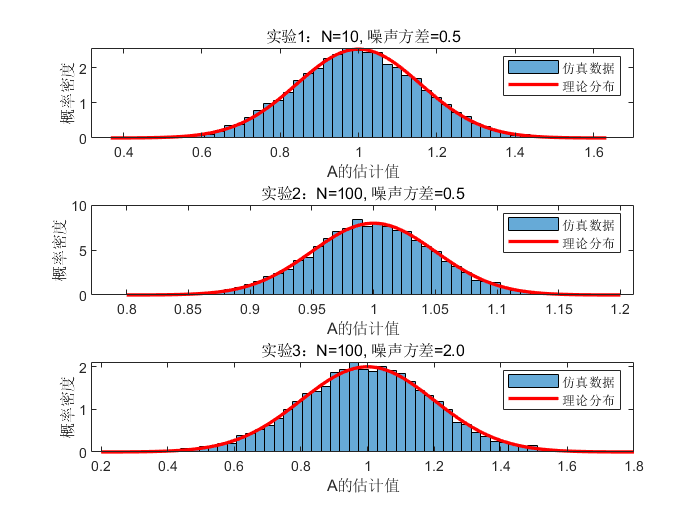
\includegraphics[width=0.8\textwidth]{image/output1.png}
    \caption{三次实验的幅度估计直方图}
\end{figure}

\subsection*{3. 实验结果分析}

\begin{itemize}
    \item 无偏性:所有实验中,实际期望 \( E[\hat{A}] \) 均接近理论期望 \( A = 1 \),验证了最大似然估计量的无偏性。轻微的偏差可能源于随机数生成的误差或仿真次数的有限性。
    \item 方差:实验结果中,实际方差与理论方差的差异较小,误差不超过1.5\%,这验证了最大似然估计量的有效性。随着采样次数 \( N \) 的增加,估计量的方差逐渐减小,估计精度提升。
\end{itemize}

\section*{未知幅度(单参量)估值(二)}

\subsection*{1. 实验原理}

假设观测信号模型为:
\[
z_i = A + n_i
\]
其中:
\begin{itemize}
    \item \( A \) 是均值为0,方差为 \( \sigma_A^2 \) 的高斯随机变量,代表未知的幅度参数。
    \item \( n_i \) 是均值为0,方差为 \( \sigma_n^2 \) 的白高斯噪声。
\end{itemize}

在本实验中,分别选取\textbf{最大似然估计(Maximum Likelihood Estimator, MLE)}和\textbf{最大后验估计(Maximum A Posteriori Estimator)}作为幅度参数 \( A \) 的估计量。

\subsubsection*{最大似然估计}

对于 \( N \) 次独立采样,观测数据为 \( \mathbf{z} = [z_1, z_2, \ldots, z_N] \)。由于噪声 \( n_i \) 独立同分布,观测值 \( z_i \) 的条件概率密度函数为:
\[
p(z_i | A) = \frac{1}{\sqrt{2\pi\sigma_n^2}} \exp\left( -\frac{(z_i - A)^2}{2\sigma_n^2} \right)
\]

因此,整个观测数据 \( \mathbf{z} \) 的似然函数为:
\[
L(A | \mathbf{z}) = \prod_{i=1}^{N} p(z_i | A) = \left( \frac{1}{\sqrt{2\pi\sigma_n^2}} \right)^N \exp\left( -\frac{1}{2\sigma_n^2} \sum_{i=1}^{N} (z_i - A)^2 \right)
\]

为了简化计算,我们对似然函数取自然对数,得到对数似然函数:
\[
\ln L(A | \mathbf{z}) = -\frac{N}{2} \ln(2\pi\sigma_n^2) - \frac{1}{2\sigma_n^2} \sum_{i=1}^{N} (z_i - A)^2
\]

为了找到 \( A \) 的最大似然估计量 \( \hat{A}_{\text{MLE}} \),我们对 \( \ln L(A | \mathbf{z}) \) 关于 \( A \) 求导,并令导数等于零:
\[
\frac{d}{dA} \ln L(A | \mathbf{z}) = -\frac{1}{2\sigma_n^2} \cdot 2 \sum_{i=1}^{N} (z_i - A) (-1) = \frac{1}{\sigma_n^2} \sum_{i=1}^{N} (z_i - A) = 0
\]
\[
\sum_{i=1}^{N} (z_i - A) = 0
\]
\[
\sum_{i=1}^{N} z_i - N A = 0
\]
\[
A = \frac{1}{N} \sum_{i=1}^{N} z_i
\]
因此,最大似然估计量为样本均值:
\[
\hat{A}_{\text{MLE}} = \frac{1}{N} \sum_{i=1}^{N} z_i
\]

\paragraph{无偏性}

验证 \( \hat{A}_{\text{MLE}} \) 的无偏性:
\[
E[\hat{A}_{\text{MLE}}] = E\left[ \frac{1}{N} \sum_{i=1}^{N} z_i \right] = \frac{1}{N} \sum_{i=1}^{N} E[z_i]
\]
由于 \( z_i = A + n_i \),且 \( E[A] = A \)(\( A \) 被视为固定常数),\( E[n_i] = 0 \),则:
\[
E[z_i] = A + E[n_i] = A
\]
因此:
\[
E[\hat{A}_{\text{MLE}}] = \frac{1}{N} \sum_{i=1}^{N} A = \frac{N A}{N} = A
\]
即 \( \hat{A}_{\text{MLE}} \) 是无偏估计量。

\paragraph{方差}

\( \hat{A}_{\text{MLE}} \) 的方差的计算如下:
\[
\text{Var}(\hat{A}_{\text{MLE}}) = \text{Var}\left( \frac{1}{N} \sum_{i=1}^{N} z_i \right) = \frac{1}{N^2} \sum_{i=1}^{N} \text{Var}(z_i) = \frac{1}{N^2} \sum_{i=1}^{N} \text{Var}(A + n_i)
\]
由于 \( A \) 是高斯分布,且 \( n_i \) 独立同分布,因此有:
\[
\text{Var}(\hat{A}_{\text{MLE}}) = \sigma_A^2 + \frac{1}{N^2} \cdot N \sigma_n^2 =\sigma_A^2 + \frac{\sigma_n^2}{N}
\]

\subsubsection*{最大后验估计}

最大后验估计(MAP)方法通过最大化后验概率 \( p(A | \mathbf{z}) \) 来估计未知参数 \( A \)。根据贝叶斯定理,后验概率 \( p(A | \mathbf{z}) \) 与似然函数 \( p(\mathbf{z} | A) \) 及先验分布 \( p(A) \) 成正比:
\[
p(A | \mathbf{z}) = \frac{p(\mathbf{z} | A) p(A)}{p(\mathbf{z})}
\]

观测数据 \( \mathbf{z} = [z_1, z_2, \ldots, z_N] \) 的似然函数为:
\[
p(\mathbf{z} | A) = \prod_{i=1}^{N} p(z_i | A) = \prod_{i=1}^{N} \frac{1}{\sqrt{2\pi\sigma_n^2}} \exp\left( -\frac{(z_i - A)^2}{2\sigma_n^2} \right)
\]
取对数似然函数:
\[
\ln p(\mathbf{z} | A) = -\frac{N}{2} \ln(2\pi\sigma_n^2) - \frac{1}{2\sigma_n^2} \sum_{i=1}^{N} (z_i - A)^2
\]

假设先验分布 \( A \) 为高斯分布:
\[
A \sim \mathcal{N}(0, \sigma_A^2)
\]
其概率密度函数为:
\[
p(A) = \frac{1}{\sqrt{2\pi\sigma_A^2}} \exp\left( -\frac{A^2}{2\sigma_A^2} \right)
\]

根据贝叶斯定理,后验分布 \( p(A | \mathbf{z}) \) 为:
\[
p(A | \mathbf{z}) \propto p(\mathbf{z} | A) p(A)
\]
将似然函数和先验分布代入:
\[
p(A | \mathbf{z}) \propto \exp\left( -\frac{1}{2\sigma_n^2} \sum_{i=1}^{N} (z_i - A)^2 \right) \exp\left( -\frac{A^2}{2\sigma_A^2} \right)
\]
对指数项进行合并:
\[
p(A | \mathbf{z}) \propto \exp\left( -\frac{1}{2\sigma_n^2} \sum_{i=1}^{N} (z_i^2 - 2z_i A + A^2) - \frac{A^2}{2\sigma_A^2} \right)
\]
整理指数项:
\[
-\frac{1}{2\sigma_n^2} \left( \sum_{i=1}^{N} z_i^2 - 2A \sum_{i=1}^{N} z_i + N A^2 \right) - \frac{A^2}{2\sigma_A^2}
\]
\[
= -\frac{1}{2\sigma_n^2} \sum_{i=1}^{N} z_i^2 + \frac{A}{\sigma_n^2} \sum_{i=1}^{N} z_i - \frac{A^2}{2\sigma_n^2} \left( N + \frac{\sigma_n^2}{\sigma_A^2} \right)
\]
忽略与 \( A \) 无关的项,得到:
\[
p(A | \mathbf{z}) \propto \exp\left( \frac{A}{\sigma_n^2} \sum_{i=1}^{N} z_i - \frac{A^2}{2} \left( \frac{N}{\sigma_n^2} + \frac{1}{\sigma_A^2} \right) \right)
\]
这表明后验分布 \( p(A | \mathbf{z}) \) 仍为高斯分布,其均值 \( \mu_p \) 和方差 \( \sigma_p^2 \) 为:
\[
\mu_p = \frac{\sigma_A^2}{\sigma_A^2 + \frac{\sigma_n^2}{N}} \cdot \frac{1}{N} \sum_{i=1}^{N} z_i
\]
\[
\sigma_p^2 = \frac{\sigma_A^4}{\sigma_A^2 N + \sigma_n^2}
\]
因此,最大后验估计量 \( \hat{A}_{\text{MAP}} \) 为后验分布的均值:
\[
\hat{A}_{\text{MAP}} = \mu_p = \frac{\sigma_A^2}{\sigma_A^2 + \frac{\sigma_n^2}{N}} \cdot \frac{1}{N} \sum_{i=1}^{N} z_i = c \cdot \hat{A}_1
\]
其中,\( \hat{A}_1 = \frac{1}{N} \sum_{i=1}^{N} z_i \) 为样本均值估计量,缩放因子 \( c \) 定义为:
\[
c = \frac{\sigma_A^2}{\sigma_A^2 + \frac{\sigma_n^2}{N}}
\]

\paragraph{无偏性}

首先验证 \( \hat{A}_{\text{MAP}} \) 的无偏性,即计算其期望值:
\[
E[\hat{A}_{\text{MAP}}] = E\left[ c \cdot \hat{A}_1 \right] = c \cdot E\left[ \hat{A}_1 \right]
\]
由于 \( \hat{A}_1 \) 为样本均值,且 \( A \) 和 \( n_i \) 均为零均值随机变量,故:
\[
E[\hat{A}_1] = E\left[ \frac{1}{N} \sum_{i=1}^{N} z_i \right] = \frac{1}{N} \sum_{i=1}^{N} E[z_i] = \frac{1}{N} \cdot N \cdot 0 = 0
\]
因此:
\[
E[\hat{A}_{\text{MAP}}] = c \cdot 0 = 0
\]
即 \( \hat{A}_{\text{MAP}} \) 是无偏估计量。

\paragraph{方差}

计算 \( \hat{A}_{\text{MAP}} \) 的方差:
\[
\text{Var}(\hat{A}_{\text{MAP}}) = \text{Var}\left( c \cdot \hat{A}_1 \right) = c^2 \cdot \text{Var}(\hat{A}_1)
\]
由于 \( \hat{A}_1 \) 为样本均值,且 \( A \) 和 \( n_i \) 独立同分布,方差为:
\[
\text{Var}(\hat{A}_1) = \sigma_A^2 + \frac{\sigma_n^2}{N}
\]
因此:

\[
\text{Var}(\hat{A}_{\text{MAP}}) = \left( \frac{\sigma_A^2}{\sigma_A^2 + \frac{\sigma_n^2}{N}} \right)^2 \cdot \left( \sigma_A^2 + \frac{\sigma_n^2}{N} \right) = \frac{\sigma_A^4}{\sigma_A^2 N + \sigma_n^2}
\]

\subsection*{2. 实验过程与结果}

实验分别进行最大似然估值和最大后验估值,主要参数如下:

\begin{itemize}
    \item 采样次数 \( N = 1000 \), 幅度方差 \( \sigma_A^2 = 0.16 \), 噪声方差 \( \sigma_n^2 = 0.25 \)
\end{itemize}

分别使用最大似然估值和最大后验估值,进行 \( 10^4 \) 次重复试验,记录每次试验的估计值 \( \hat{A} \),并计算其均值和方差,与理论值进行比较。

\subsubsection*{最大似然估值结果}

\begin{itemize}
    \item 理论期望:\( E[\hat{A}] = 0.0000 \)
    \item 实际期望:\( E[\hat{A}] = 0.0016 \)
    \item 理论方差:\( \text{Var}(\hat{A}) = 0.160250 \)
    \item 实际方差:\( \text{Var}(\hat{A}) = 0.159057 \)
\end{itemize}

\subsubsection*{最大后验估值结果}

\begin{itemize}
    \item 理论期望:\( E[\hat{A}] = 0.0000 \)
    \item 实际期望:\( E[\hat{A}] = 0.0016 \)
    \item 理论方差:\( \text{Var}(\hat{A}) = 0.159750 \)
    \item 实际方差:\( \text{Var}(\hat{A}) = 0.158561 \)
\end{itemize}

同时,绘制每个实验中$\hat A$的估计值的直方图,并叠加理论的正态分布曲线,以验证估计量的分布特性。

\begin{figure}[H]
    \centering
    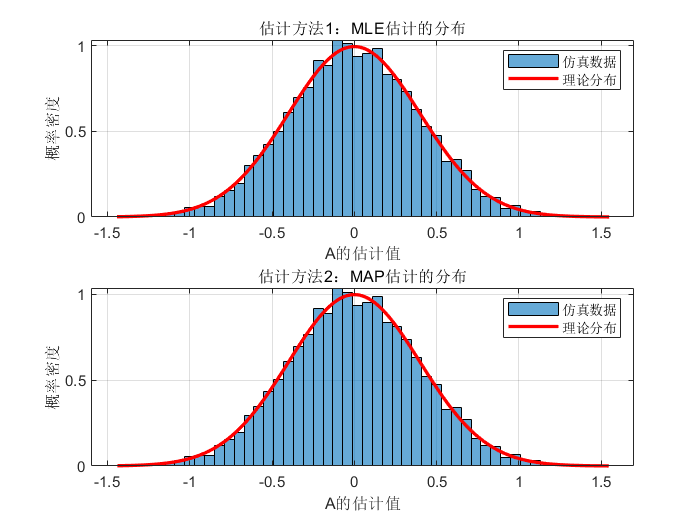
\includegraphics[width=0.8\textwidth]{image/output2.png}
    \caption{两种估值的幅度估计直方图}
\end{figure}

\subsection*{3. 实验结果分析}

\begin{itemize}
    \item 
\end{itemize}


\section*{三、未知幅度(单参量)估值(三)}

\subsection*{1. 实验原理}

假设观测信号模型为:
\[
    z_i = A\cos(\omega t) + n
\]
其中幅度和噪声与(二)中相同。本实验采用与(二)相同的最大似然估计和最大后验估计方法,分别估计幅度参数 \( A \)。
估值公式分别如下:

\[
\hat{A}_{MLE} = \frac{1}{N} \sum_{i=1}^{N} z_i
\]
\[
\hat{A}_{\text{MAP}} = \frac{\sigma_A^2}{\sigma_A^2 + \frac{\sigma_n^2}{N}} \cdot \frac{1}{N} \sum_{i=1}^{N} z_i 
\]
\subsection*{2. 实验内容与结果}

\begin{itemize}
    \item 频率$\omega = 100 $Hz, 采样次数 \( N = 1000 \), 幅度方差 \( \sigma_A^2 = 0.16 \), 噪声方差 \( \sigma_n^2 = 0.25 \)
\end{itemize}

分别使用最大似然估值和最大后验估值,进行 \( 10^4 \) 次重复试验,记录每次试验的估计值 \( \hat{A} \),并计算其均值和方差,与理论值进行比较。

\subsubsection*{最大似然估值结果}

\begin{itemize}
    \item 理论期望:\( E[\hat{A}] = 0.0000 \)
    \item 实际期望:\( E[\hat{A}] = 0.0029 \)
    \item 理论方差:\( \text{Var}(\hat{A}) = 0.160250 \)
    \item 实际方差:\( \text{Var}(\hat{A}) = 0.408594 \)
\end{itemize}

\subsubsection*{最大后验估值结果}

\begin{itemize}
    \item 理论期望:\( E[\hat{A}] = 0.0000 \)
    \item 实际期望:\( E[\hat{A}] = 0.0029 \)
    \item 理论方差:\( \text{Var}(\hat{A}) = 0.159750 \)
    \item 实际方差:\( \text{Var}(\hat{A}) = 0.407320 \)
\end{itemize}

同时,绘制每个实验中$\hat A$的估计值的直方图,并叠加理论的正态分布曲线,以验证估计量的分布特性。

\begin{figure}[H]
    \centering
    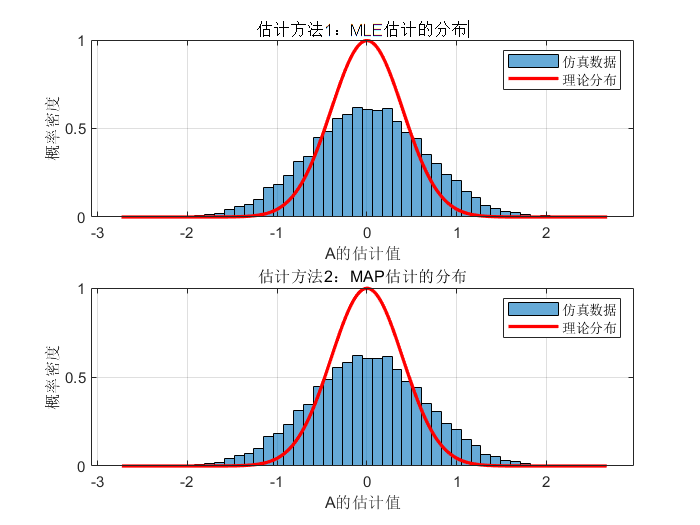
\includegraphics[width=0.8\textwidth]{image/output3.png}
    \caption{两种估值的幅度估计直方图(正弦信号)}
\end{figure}

\subsection*{3. 实验结果分析}

在信号模型 $z_i = A \cos(\omega t) + n$ 中,由于余弦函数 $\cos(\omega t)$ 的周期性和非零点放大效应,导致在 $\cos(\omega t)$ 靠近零时,噪声 $n$ 被放大,进而影响了估计值的精度。
特别是在计算样本均值或 MAP 估计时,这种效应会显著增加估计值的方差.

\section*{波士顿房价预测实验}

\subsection*{1. 实验原理}

波士顿房价预测是机器学习领域经典的回归预测问题。本实验中,通过使用树回归回归算法进行房价趋势分析。

\subsection*{2. 实验内容与结果}

实验主要进行流程如下:

\paragraph{数据准备}

数据集包含1460个波士顿房屋样本,79个关于描述房屋的特征。根据这些数据特征预测房屋的最终售价,即预测测试集中每个房屋ID对应的SalePrice字段的数值。
数据集中可能包含部分缺失、类型不对应,以及值异常的情况,进行数据预处理。
经偏度和峰度计算并$\ln$转化后,'SalePrice'概率分布图如下,可以看到大致服从正态分布。

\begin{figure}[H]
    \centering
    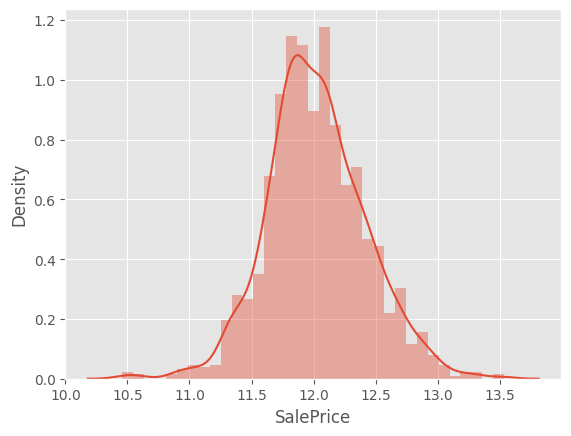
\includegraphics[width=0.7\textwidth]{image/output4-2.png}
    \caption{SalePrice分布情况}
\end{figure}

同时,绘制qq图如下,用于体现SalePrice服从正态分布的情况,可以看到蓝色部分接近直线,正态性明显。

\begin{figure}[H]
    \centering
    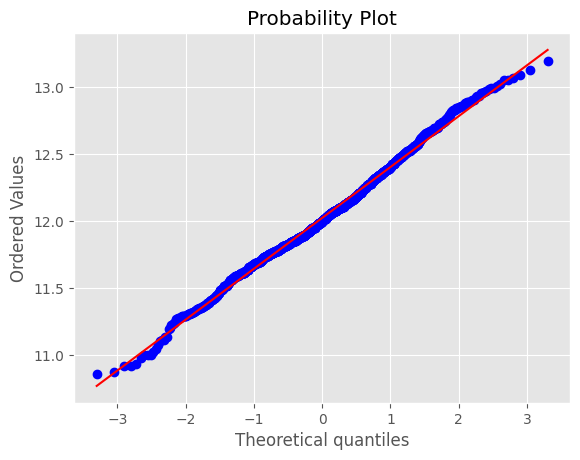
\includegraphics[width=0.7\textwidth]{image/output4-3.png}
    \caption{SalePrice qq图}
\end{figure}

\paragraph{特征工程}

主要包含特征选取、构建新的特征、特征融合的步骤。

首先通过相关性分析,通过指标筛选重要特征,再对离散特征进行one-hot编码,并绘制热力图如下。

\begin{figure}[H]
    \centering
    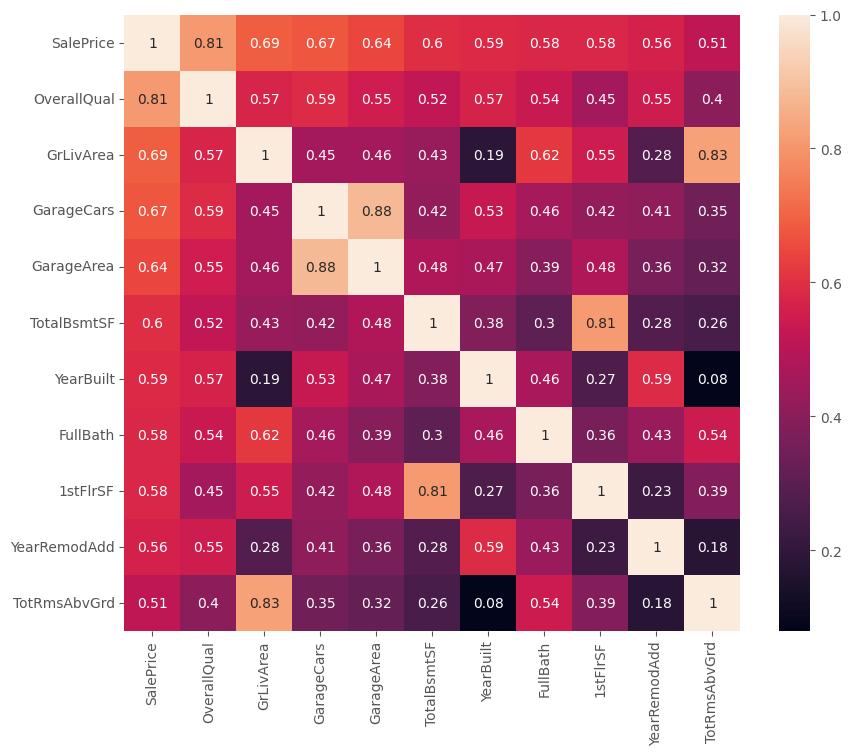
\includegraphics[width=0.7\textwidth]{image/output4-4.png}
    \caption{特征相关性热力图}
\end{figure}

对面积特征进行分析:通过观察异常值进行筛选,并验证是否服从正态分布。对于偏度大于0.75的通过$\ln(x+1)$转换,使其接近正态分布效果。
同时,通过绘制直方图,查看不同月份房子销售量, 作为非线性特征,如图所示。

\begin{figure}[H]
    \centering
    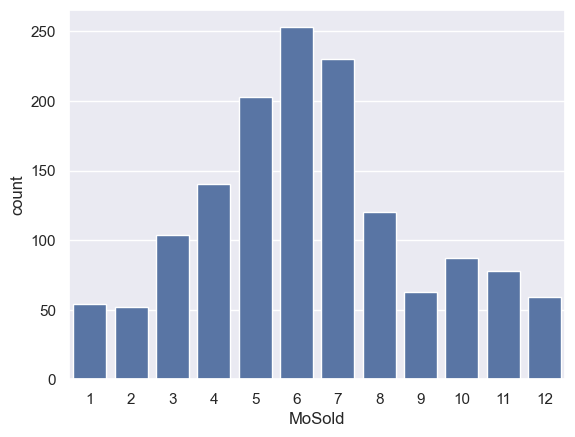
\includegraphics[width=0.7\textwidth]{image/output4-6.png}
    \caption{不同月份房子销售量}
\end{figure}

通过方差分析选取靠前的25个重要特征,进行特征融合,并分别绘制Total Area和Total House 回归图如下,用于查看构建的面积特征效果。
同时对其他特征也进行特征融合,用以减少后续数据维度,提高模型训练速度。

\begin{figure}[H]
    \centering
    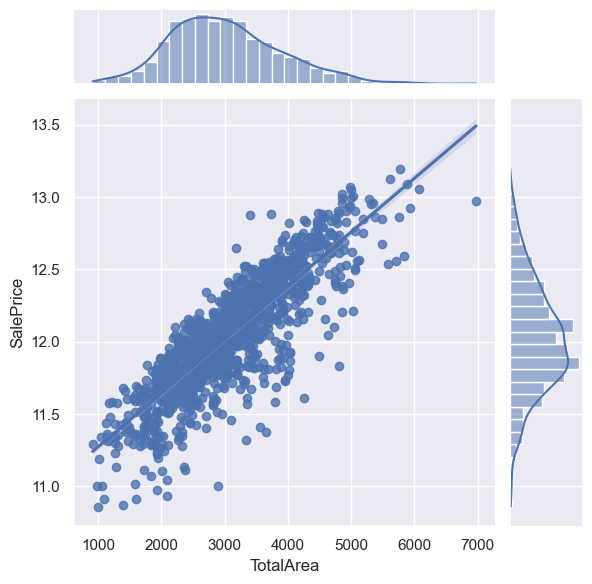
\includegraphics[width=0.7\textwidth]{image/output4-8.png}
    \caption{Total Area 回归图}
\end{figure}    

\begin{figure}[H]
    \centering
    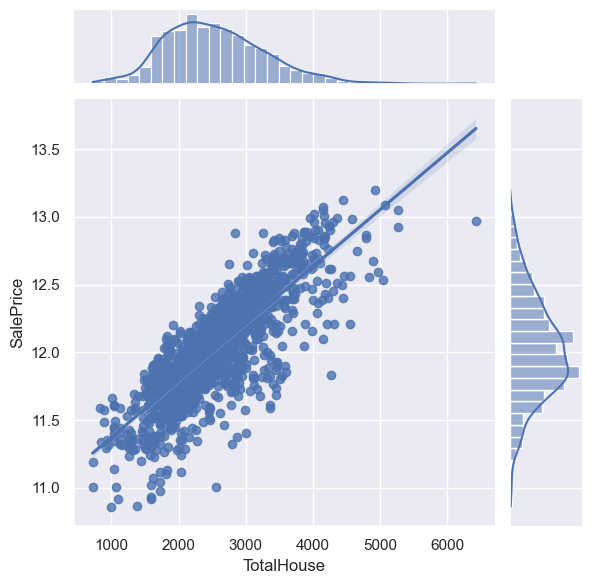
\includegraphics[width=0.7\textwidth]{image/output4-7.png}
    \caption{Total House 回归图}
\end{figure}  

\paragraph{模型训练}

首先将数据进行标准化,将数据顺序打乱,进行5折交叉验证,将均方根误差作为评判标准,采用GBDT算法构建树回归算法模型,进行调参,使根均方误差最小化。

使用GBDT算法构建树回归算法模型如下:

\begin{lstlisting}
GBoost = GradientBoostingRegressor(
                        n_estimators=3000, learning_rate=0.005,
                        max_depth=4, max_features='sqrt',
                        min_samples_leaf=15, min_samples_split=10, 
                        loss='huber', random_state =5)
\end{lstlisting}

并按照80\%训练集,20\%测试集进行拟合效果测试,结果如下:

\begin{figure}[H]
    \centering
    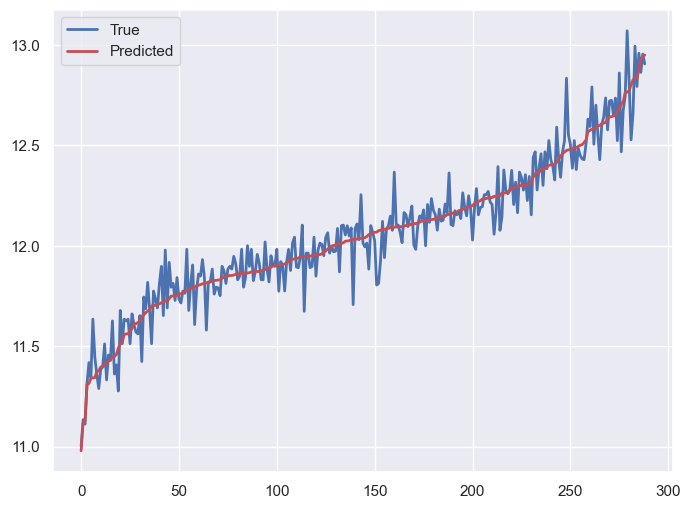
\includegraphics[width=0.7\textwidth]{image/output4-9.png}
    \caption{GBDT算法拟合效果}
\end{figure} 

使用Xgboost算法构建回归算法模型如下:

\begin{lstlisting}
Xgboost = xgb.XGBRegressor(
                    colsample_bytree=0.36, gamma=0.042, 
                    learning_rate=0.05, max_depth=3, 
                    min_child_weight=1.88, n_estimators=2200,
                    reg_alpha=0.4640, reg_lambda=0.8571,
                    subsample=0.5213, silent=1,
                    random_state = 1, nthread = -1)
\end{lstlisting}

与上面相同,对拟合效果进行测试,结果如下:

\begin{figure}[H]
    \centering
    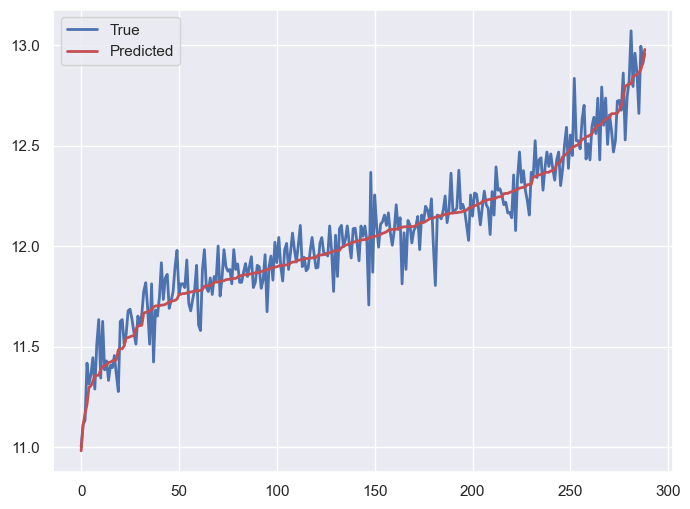
\includegraphics[width=0.7\textwidth]{image/output4-10.png}
    \caption{Xgboost算法拟合效果}
\end{figure} 

\subsection*{3. 实验结果分析}

参量估值问题和回归预测问题有着以下相同点和不同点:

\subsubsection*{共同点}
\begin{itemize}
    \item 两者都以估计目标变量为核心,强调误差的最小化;
    \item 模型性能均受噪声、样本数量和数据质量的影响;
    \item 在数据预处理和优化过程中,特征归一化或噪声过滤是常见手段。
\end{itemize}

\subsubsection*{不同点}
\begin{itemize}
    \item \textbf{目标维度}:参量估值问题通常处理单一或低维参数,而回归预测问题处理高维特征与目标变量的映射关系;
    \item \textbf{方法复杂度}:参量估值问题通常依赖解析解或优化算法,而回归预测问题需要更复杂的机器学习算法;
    \item \textbf{结果解释}:参量估值问题侧重数学意义上的精确性(如无偏性、最小方差),而回归预测问题更注重预测精度和泛化能力。
\end{itemize}

\newpage

\begin{thebibliography}{99}

    \bibitem{Schonhoff2007}
    T.A. Schonhoff \& A.A. Giordano, \textit{Detection and Estimation: Theory and its Applications}. Pearson Education, Inc., 2007. (信号检测与估计——理论与应用,关欣等译,电子工业出版社,2012年).
    
    \bibitem{Srinath1996}
    M.D. Srinath, P.K. Rajasekaran \& R. Viswanathan, \textit{Introduction to Statistical Signal Processing with Applications}. Prentice Hall, 1996.  
    
    \bibitem{Kay1993}
    Steven M. Kay, \textit{Fundamentals of Statistical Signal Processing, Volume I: Estimation Theory} (©1993) \& \textit{Volume II: Detection Theory} (©1998). Pearson Education. (《统计信号处理基础:估计与检测理论(卷 I、卷 II合集)》,罗鹏飞等译,电子工业出版社,2023年).  
    
    \bibitem{Candy2016}
    James V. Candy, \textit{Bayesian Signal Processing: Classical, Modern, and Particle Filtering Methods} (2nd ed.). John Wiley \& Sons, Inc., 2016. (宗华等译,哈尔滨工业大学出版社,2023年).  
    
    \bibitem{VanTrees2013}
    Harry L. Van Trees, Kristine L. Bell, with Zhi Tian, \textit{Detection Estimation and Modulation Theory, Part I: Detection, Estimation, and Filtering Theory} (2nd ed.). John Wiley \& Sons, Inc., 2013.  
    
    \bibitem{ChatGPT2024}
    ChatGPT by OpenAI (2024). Personal communication and consultation for generating LaTeX formatting, experimental methodology, and model evaluation strategies. OpenAI, \url{https://www.openai.com}.  
    
\end{thebibliography}
    
    

\end{document}